\documentclass[fontsize=12pt, a4paper]{scrartcl}
\let\stdsection\section 	% neue seite für neues kapitel
\renewcommand\section{\newpage\stdsection} 

% ### variables

\def \var_single_plot_width {0.49}
\def \var_double_plot_width {0.49}

% ### literaturverzeichnis
\usepackage[sorting=none]{biblatex}
\addbibresource{sim_axelsson.bib}

% ### sprachpakete
\usepackage[ngerman]{babel} % Deutsche Sprachanpassungen
\usepackage[T1]{fontenc}    % Silbentrennung bei Sonderzeichen
\usepackage[utf8]{inputenc} % Direkte Angabe von Umlauten im Dokument.
    
% ### grafiken   
\usepackage{graphicx}		% Zur Darstellung von Bildern
\usepackage{subcaption}
\usepackage{float}			% platziert figures am gewünschten platz
\usepackage[export]{adjustbox}% http://ctan.org/pkg/adjustbox
\usepackage{svg}
\usepackage{amsmath}
\usepackage{bm}

% ### matplotlib plots
\usepackage{pgf}
\usepackage{lmodern}% http://ctan.org/pkg/lm
%\usepackage{tikz}
\usepackage{pgfplots}
\pgfplotsset{width=10cm,compat=1.9}
%\pgfplotsset{compat=newest}

\usepackage{csquotes}

\usepackage[parfill]{parskip}

% ### curcuits
\usepackage{tikz}
\usetikzlibrary{arrows}
\usepackage[RPvoltages]{circuitikz}

% ### titleseite
\usepackage{titling}
\title{Systemmodelierung einer Membranpumpe für die Mikro-Fluidik}
\author{Kristjan Axelsson, Timo Stubler}
\date{\today}               

% ### fancy features
\usepackage{hyperref}

\begin{document}
\pagenumbering{gobble}		% turn off page numbers
\begin{titlingpage}
\begin{center}
\begin{figure}[H]
    \centering
    \begin{subfigure}[B]{0.2\textwidth}
        
\includegraphics[width=\textwidth, valign=t]{bilder/Logo_MNM_EN_Farbe_ohneHM (1).png}
    \end{subfigure}
    \begin{subfigure}[B]{0.45\textwidth}
        
\includegraphics[width=\textwidth, valign=t]{bilder/Hochschule_Muenchen_Logo.png}
    \end{subfigure}
\end{figure}
\setcounter{figure}{0}
\vspace{2cm}
\begin{large} 
\textbf{\thetitle} \\
\end{large}
\vspace{1cm}
\theauthor\\
\vspace{1cm}
Hochschule München \\
Fakultät für angewandte Wissenschaften und Mechatronik \\
\vspace{1cm}
\thedate
\end{center}
\end{titlingpage}

\tableofcontents            % Inhaltsverzeichnis anlegen

% quelle \cite{pedrotti} \\
% siehe Abb. \ref{fig_detector_test} \\
% siehe Kap. \ref{fazit}

\section{Einleitung}
\pagenumbering{arabic}		% turn on page numbers



\section{Theorie}

Im Folgenden wird die Modellierung der Membranpumpe besprochen. Der Antrieb der Pump wird durch einen Piezoaktor realisiert. Dieser wird über einen Wechselspannung betrieben und erzeugt so abwechselnd einen Über- bzw. Unterdruck in der Pumpkammer. Die Ventile sind passive Klappenventile welche nur in eine Richtung öffnen. Je nach Anordnung dient dieses Ventil einmal als Auslass und einmal als Einlass. Die Klappenventile sind über einen Schlauch jeweils mit einem Reservoir verbunden.

Im Folgenden werden zwei Modelle vorgestellt. Das erste Besteht aus der Pumpkammer mit einem Klappenventil und einer Zuleitung welche an eine Reservoir angeschlossen ist (einarmiges Model). Diese Model dient der Untersuchung der Ventile auf Leckströme und der Untersuchung der Zuleitungen auf deren Geometrie. Das zweite Model umfasst die Gesamte Pumpe welche auf ihre Funktionsweise bezogen auf Gegendruck und Antriebsfrequenz untersucht wird (zweiarmiges Model).

Für die Simulation wird ein fluidisches Ersatzmodel verwendet [Quelle Skript]

\[ Widerstand \:\widehat{=}\:  Strömungswiderstand = \biggl[\frac{m^3/s}{Pa}\biggr] \]
\[ Kapazität  \:\widehat{=}\:  fluidische Kapazität = \biggl[\frac{m^3}{Pa}\biggr] \]
\[ Spannung  \:\widehat{=}\:  Druck = [Pa] \]

\[ P = R\dot{V} \]
\[ P = \frac{V}{C} \]
\[ P = P \]

\subsection{Reservoir}
Das Reservoir wird als unendlich groß angenommen und daher mit einem Konstanten Druck modelliert.


\[ Pr = Umgebungsdruck \]

Die Zuleitung wird durch einen einfachen Strömungswiderstand modelliert. Da diese Strömung als laminar betrachtet wird ist der Strömungswiderstand über das Gesetz von Hagen-Poiseuille zu beschreiben

\begin{equation}
	\dot{V} = \frac{pi * r^4 * dP}{8* eta *l}
\end{equation}

\begin{equation}
	R = \frac{8* eta *l}{pi * r^4}
\end{equation}

\subsection{Klappenventile}

Die Klappenventile werden durch einen Widerstand beschrieben welcher vom Druck abhängt. Für Drücke > 0 ist das Ventil geöffnent. Für Drücke < 0 ist das Ventil geschlossen. Die Widerstände für den geöffneten und geschlossenen Zustand werden über das oben beschriebene Gesetz von Hagen-Poiseuille beschrieben.

[Evtl. Grafik]

\subsection{Pumpkammer}
Real wird die Auslenkung der Pumpkammer durch Anlegen eines elektrischen Signales erzeugt. Dadurch verändert sich der Druck in der Pumpkammer, sowie dessen Kapazität. Die Pumpkammer ist in erster Näherung durch einen Kolben zu beschreiben. Die Höhe der Druckamplitude wird durch einen Proportionalitätsfaktor von der Spannung abhängig gemacht, ebenso die fluidische Kapazität. Die Extremwerte für Druck und Kapazität der Pumpkammer werden aus [Quelle ??] entnommen.

Die Trägheit der Pumpe wird über ein RC angenähert.

Der Wert für die Zeitkonstante wird abgeschätzt.

Hinterlegung der Kennlinie um in der Simulation zeitabhängige Werte für Pumpkammerdruck und -Kapazität zu bekommen.

[Kennlinien der Pumkammer]

\begin{figure}[H]
	\centering
	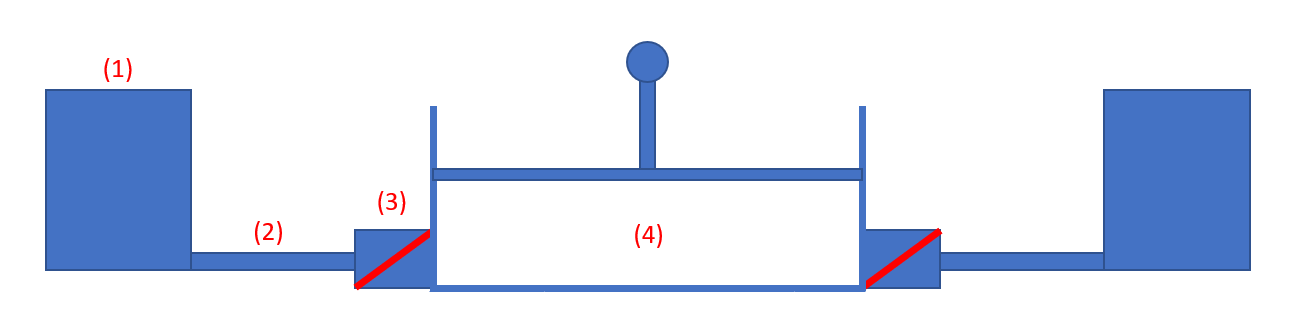
\includegraphics[width=0.98\textwidth]{bilder/theorie/pumpe_prinzipskizze.PNG}
	\caption{1) Reservoir 2) Zulauf 3) Ventil 4) Pumpkammer}
\end{figure}


\section{Modellierung}

Im Folgenden wird die Modellierung des Einzelstrangs und des Gesamtsystems Pumpe behandelt.
Wie bereits erwähnt, werden elektrische Ersatzschaltbilder herangezogen, welche dann mithilfe der elektrisch-fluidischen Analogiegesetze untersucht werden.

\subsection{Einzelstrang}

Das Gesamtsystem Pumpe kann in zwei Einzelstränge (ein-, ausleitend) unterteilt werden, welche jeweils einen in sich geschlossenen Kreislauf im Ersatzschaltbild darstellen.
Die Betrachtung eines Strangs kann analog auf den anderen übertragen werden. Folglich wird hier nur ein Strang erläutert.

\begin{center}
	\includesvg[scale = 0.6]{bilder/circuits/single_branch}
\end{center}

Der Eingangsdruck ($U_{in}$), der Reservoir-bedingt anliegt, bildet mit dem durch den Piezoaktor erzeugten Kammerdruck ($U_{Signal}(t)$) eine Druckdifferenz. Nach Hagen-Poiseuille resultiert daraus ein Volumenstrom in eine vom Vorzeichen der Druckdifferenz ($U_{Signal}(t)-U_{in}$) vorgegebene Richtung. Der Leitungswiderstand ($R_{T}$) und der Ventilwiderstand ($R_{V}$) begrenzen die resultierenden Volumenströme. Dabei beherbergt das Modell des Ventils eine Abhängigkeit von der Druckdifferenz. Im gezeigten Einzelstrang ist der Ventilwiderstand für negative Druckdifferenzen gering, für positive Druckdifferenzen sehr hoch, sodass das Ventil in diese Richtung schließt. Am Ende des Einzelstranges befindet sich die Pumpkammer und die Quelle des Drucksignals. Das Aufnahmevermögen der Pumpkammer wird durch ein Kondensatorelement beschrieben. Die hierin stattfindenden Druckänderungen ($P_{C}$) gilt es zeitlich zu ermitteln.

Dazu wird die Differentialgleichung mithilfe des Kirchhoff´schen Gesetz (Maschenbedingung) ermittelt:

\begin{equation}
	U_{Signal}(t) - U_{in} + U_{C} + U_{R_{T}} + U_{R_{V}} = 0
\end{equation}

\begin{equation}
	\dot{U}_{C} = \frac{1}{C_{C}} * \frac{-U_{Signal}(t)+U_{in}-U_{C}}{R_{T}+R_{V}}
\end{equation}

\begin{equation}
	P_{Signal}(t) - P_{in} + P_{C} + P_{R_{T}} + P_{R_{V}} = 0
\end{equation}

\begin{equation}
	\dot{P}_{C} = \frac{1}{C_{C}} * \frac{-P_{Signal}(t)+P_{in}-P_{C}}{R_{T}+R_{V}}
\end{equation}


\subsection{Gesamtsystem}

Die gezeigten Einzelstränge sind über die Pumpkammer gekoppelt und ergeben das Gesamtsystem (siehe Abbildung).


\begin{center}
	\includesvg[scale = 0.75]{bilder/circuits/first_order_circuit}
\end{center}

Um einen Volumenstrom zwischen den beiden Reservoirs zu erreichen sind die Ventile gegensätzlich angeordnet, so dass diese bei Änderung der Druckdifferenz abwechselnd schalten. 

Um das System analytisch beschreiben zu können, wird wieder die Differentialgleichung hergeleitet. Dabei muss neben der Maschenbedingungn auch die Knotenbedingung berücksichtigt werden:

\begin{equation}
	I_{C} = I_{in} + I_{out}
\end{equation}

\begin{equation}
	U_{Signal}(t) - U_{in} + U_{C} + U_{R_{T_{in}}} + U_{R_{V_{in}}} = 0
\end{equation}

\begin{equation}
	U_{Signal}(t) - U_{out} + U_{C} + U_{R_{T_{out}}} + U_{R_{V_{out}}} = 0
\end{equation}

\begin{equation}
	\dot{U}_{C} = - \frac{1}{C_{C}} * \biggl[\frac{U_{Signal}(t)-U_{in}+U_{C}}{R_{T_{in}}+R_{V_{in}}} + \frac{U_{Signal}(t)-U_{out}+U_{C}}{R_{T_{out}}+R_{V_{out}}}\biggr]
\end{equation}

\begin{equation}
	\dot{P}_{C} = - \frac{1}{C_{C}} * \biggl[\frac{P_{Signal}(t)-P_{in}+P_{C}}{R_{T_{in}}+R_{V_{in}}} + \frac{P_{Signal}(t)-P_{out}+P_{C}}{R_{T_{out}}+R_{V_{out}}}\biggr]
\end{equation}
Wie schon angedeutet, hängen die Werte $R_{V_{in}}(P_{V_{in}})$ und $R_{V_{out}}(P_{V_{out}})$ von der über dem jeweiligen Ventil anliegenden Druckdifferenz ab. Diese wird über einen Spannungsteiler ermittelt, sodass die Simulation in jedem Zeitschritt den druckbasierten Widerstandswert der Ventile anpassen kann.

\section{Simulation}

Diese Kapitel umfasst die Untersuchungen des einarmigen und zweiarmigen Models der Membranpumpe

Beschreibung ODEINT

Beschreibung wie Abhängigkeit Ventilwiderstand <-> Druckdifferenz gelöst ist. (Denke da haben wir einen Bug :D)

\subsection{Zuleitungen}

\begin{figure}[H]
	\centering
	\begin{subfigure}[H]{0.48\textwidth}
		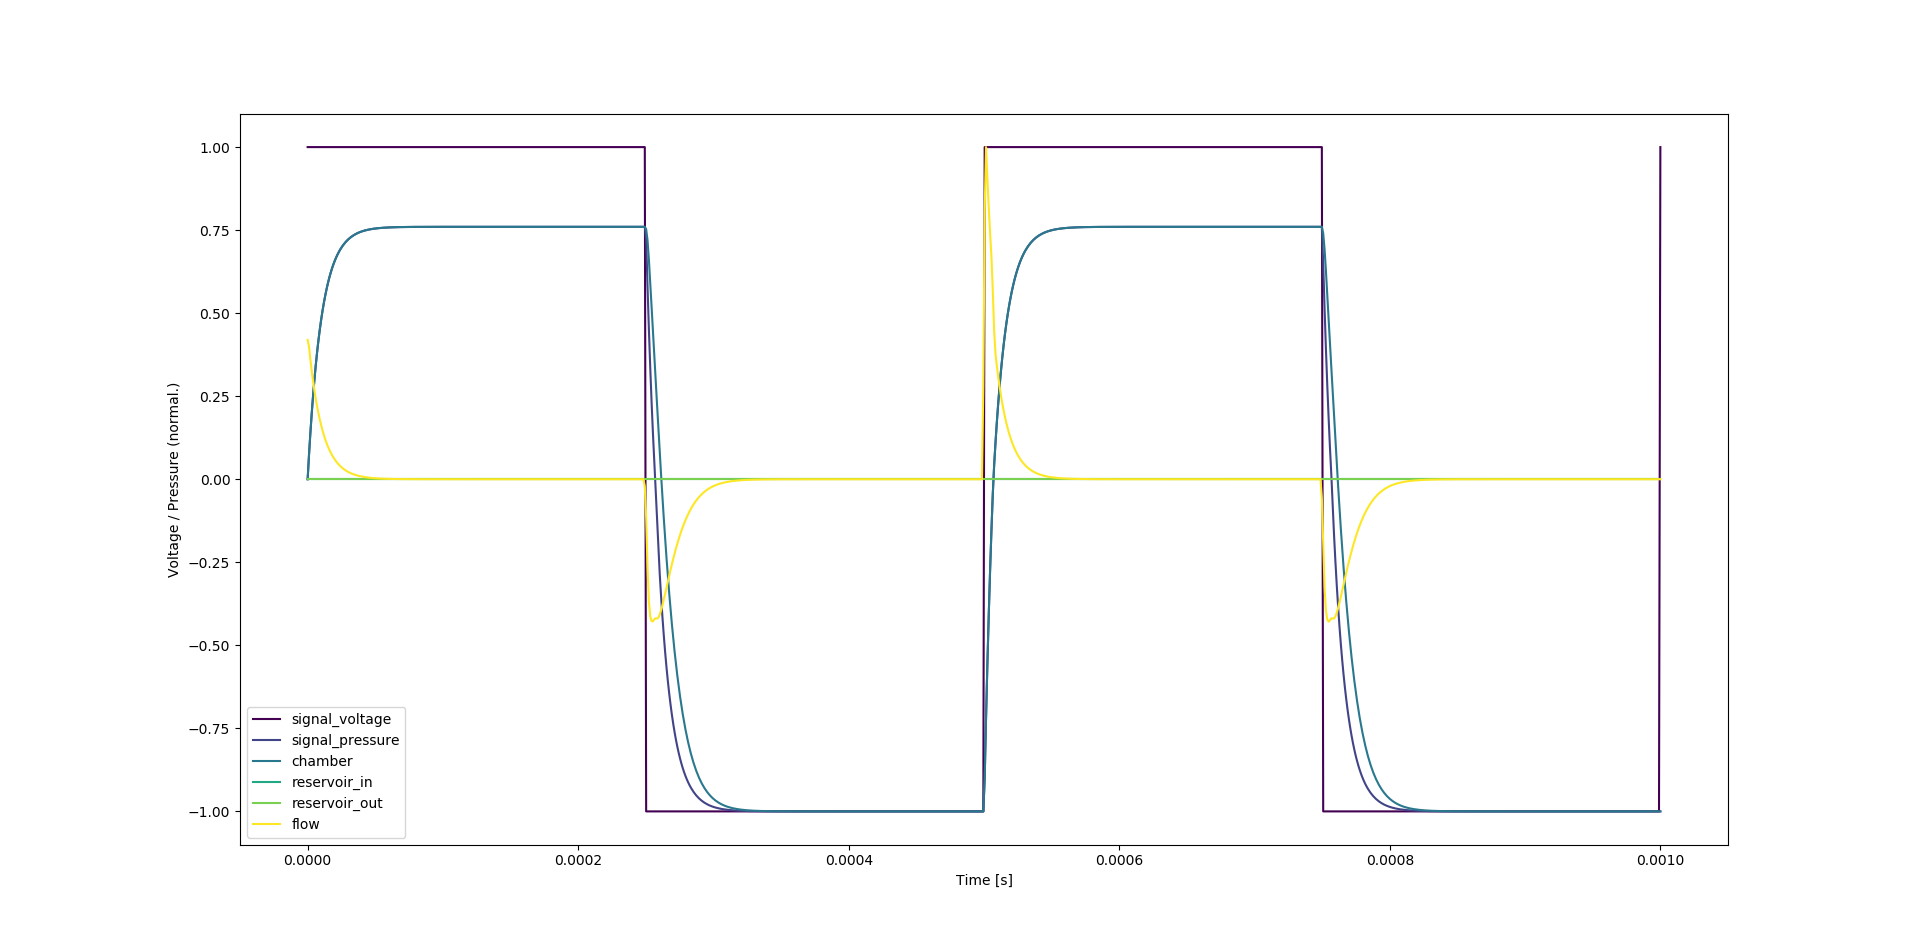
\includegraphics[width=\textwidth, valign=t]{bilder/tubelength/tl_in_branch_singlesweep.png}
		\caption{•}
	\end{subfigure}
	\begin{subfigure}[H]{0.48\textwidth}
		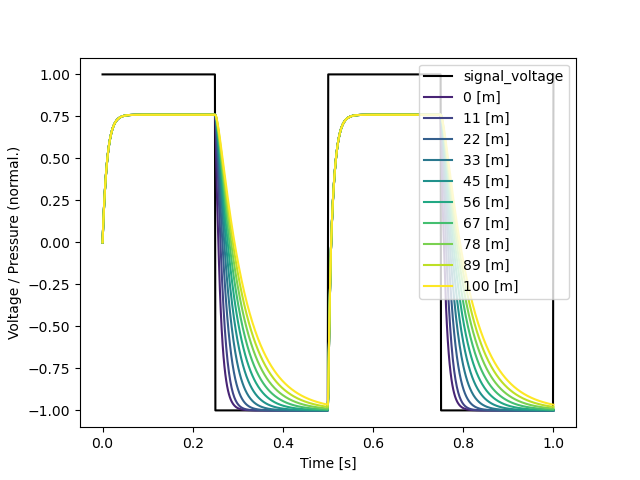
\includegraphics[width=\textwidth, valign=t]{bilder/tubelength/tl_in_branch_multisweep.png}
		\caption{•}
	\end{subfigure}
	\caption{•}
\end{figure}

\begin{figure}[H]
	\centering
	\begin{subfigure}[H]{0.48\textwidth}
		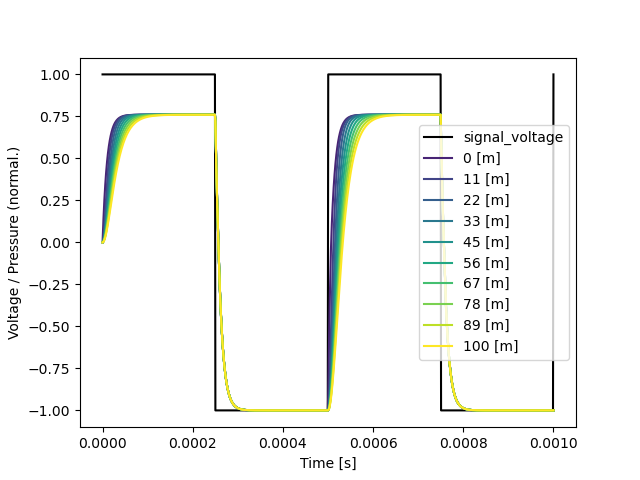
\includegraphics[width=\textwidth, valign=t]{bilder/tubelength/tl_out_branch_multisweep.png}
		\caption{•}
	\end{subfigure}
	\begin{subfigure}[H]{0.48\textwidth}
		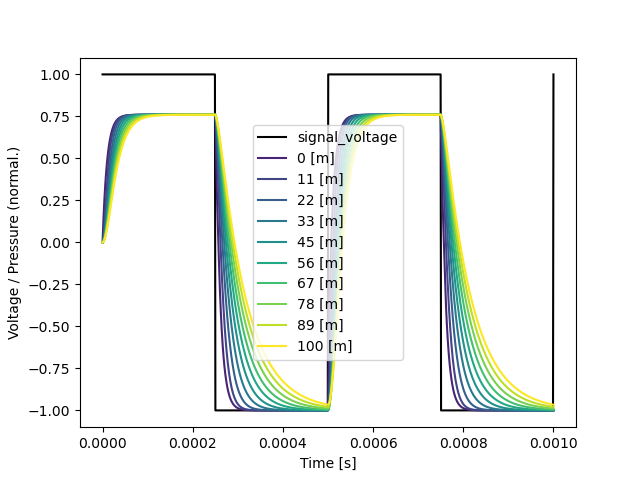
\includegraphics[width=\textwidth, valign=t]{bilder/tubelength/tl_both_branch_multisweep.png}
		\caption{•}
	\end{subfigure}
	\caption{•}
\end{figure}

\begin{figure}[H]
	\centering
	\begin{subfigure}[H]{0.48\textwidth}
		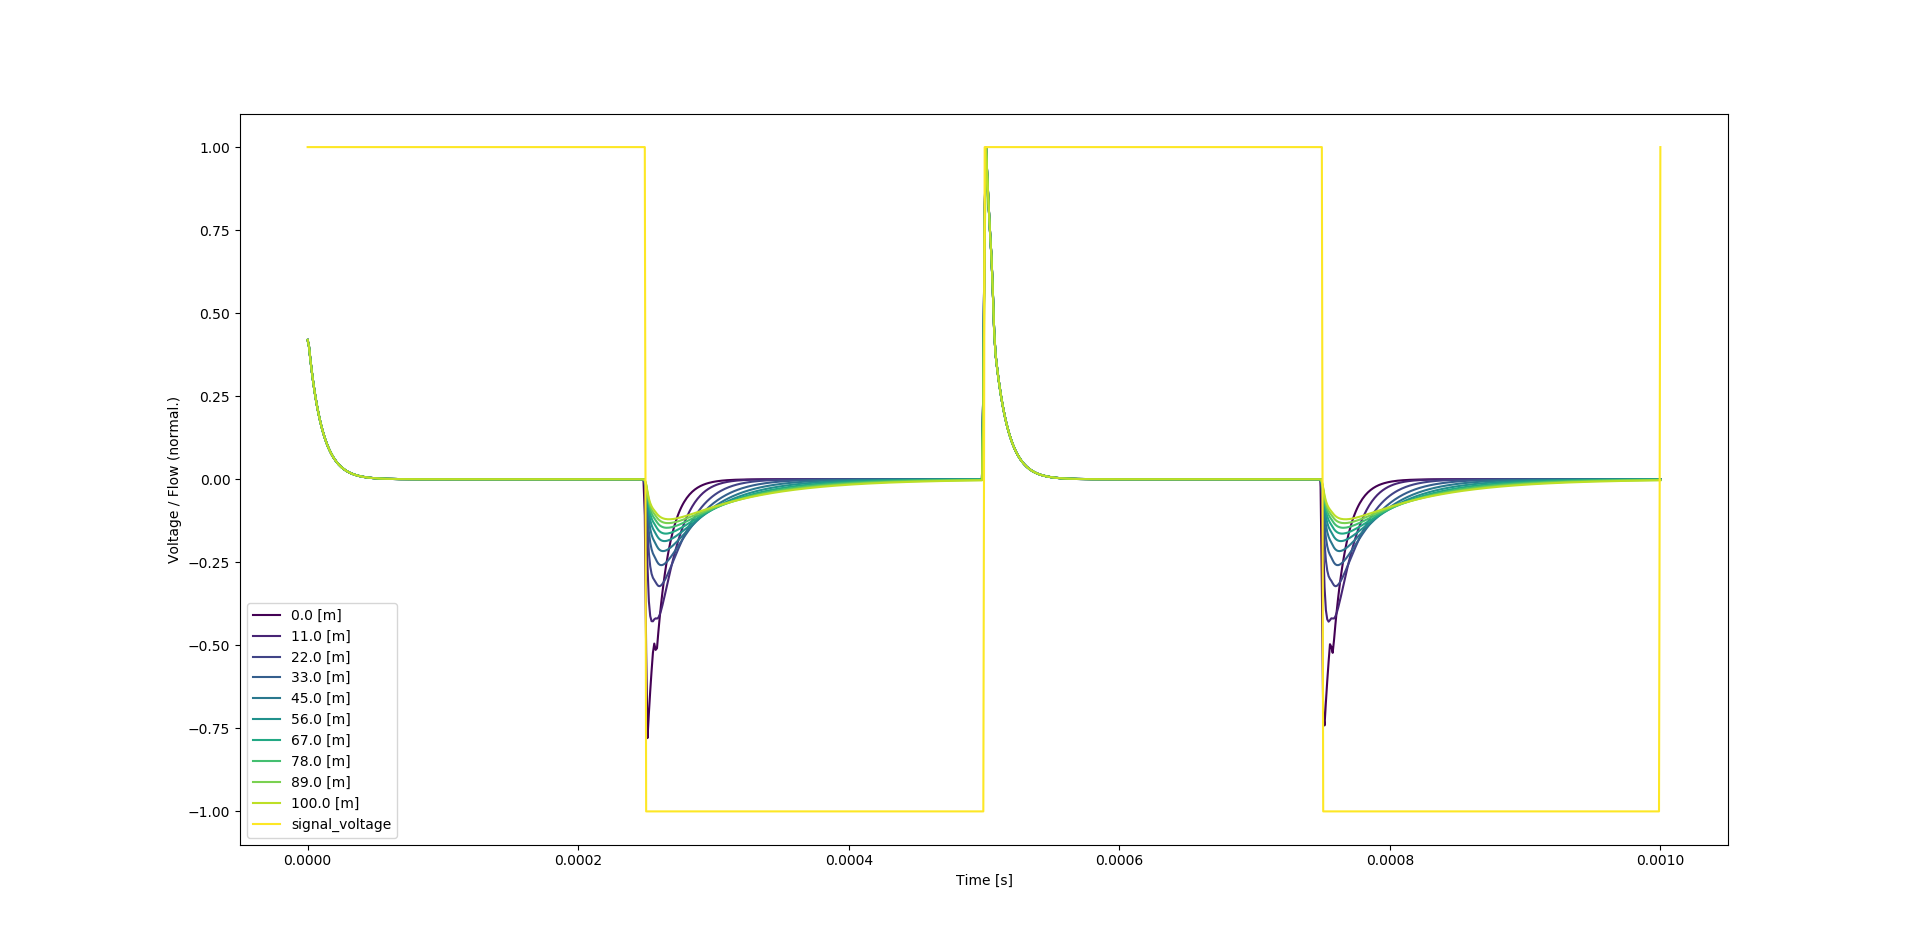
\includegraphics[width=\textwidth, valign=t]{bilder/tubelength/tl_in_branch_multisweep_flow.png}
		\caption{•}
	\end{subfigure}
	\begin{subfigure}[H]{0.48\textwidth}
	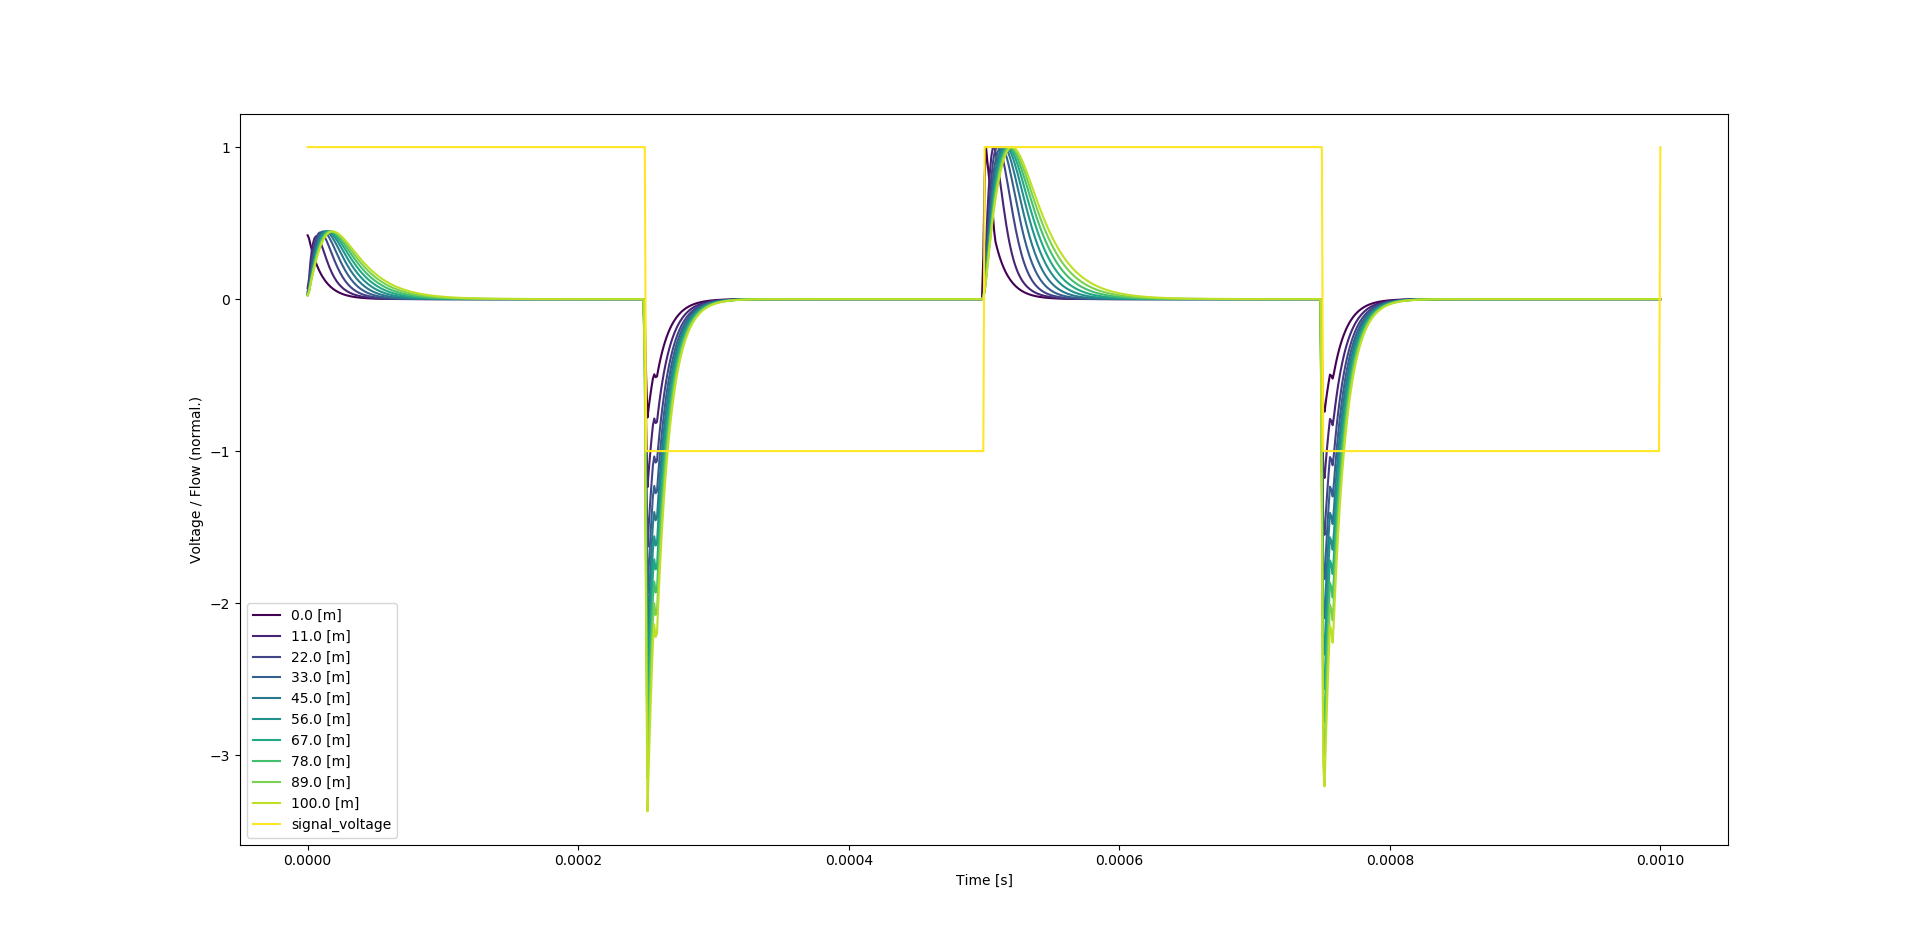
\includegraphics[width=\textwidth, valign=t]{bilder/tubelength/tl_out_branch_multisweep_flow.png}
	\caption{•}
	\end{subfigure}
	\begin{subfigure}[H]{0.48\textwidth}
		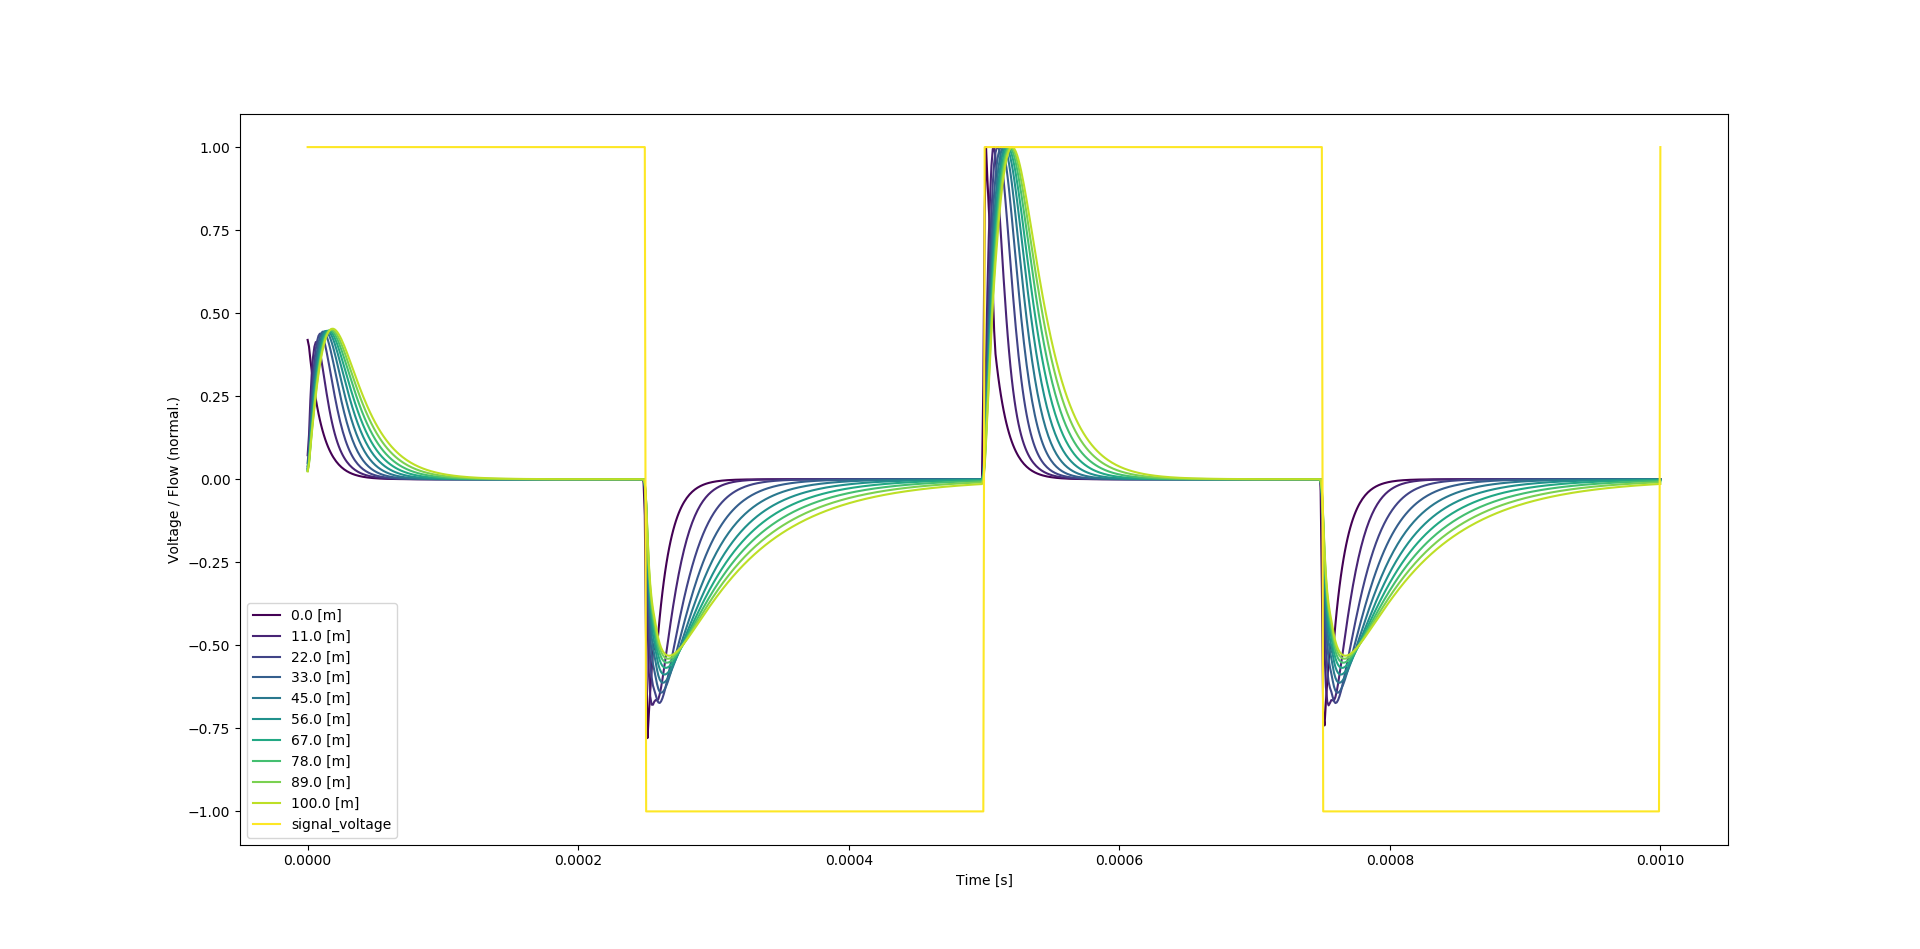
\includegraphics[width=\textwidth, valign=t]{bilder/tubelength/tl_both_branch_multisweep_flow.png}
		\caption{•}
	\end{subfigure}
	\caption{•}
\end{figure}

\subsection{Leckströme}

\begin{figure}[H]
	\centering
	\begin{subfigure}[H]{0.48\textwidth}
		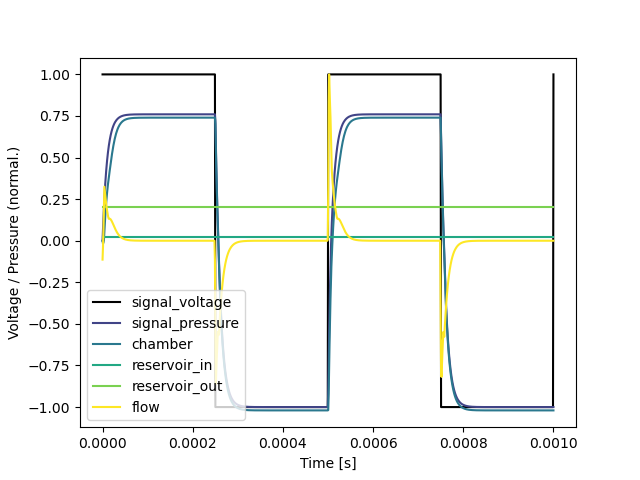
\includegraphics[width=\textwidth, valign=t]{bilder/velveresistance/vr_in_branch_singlesweep.png}
		\caption{•}
	\end{subfigure}
	\begin{subfigure}[H]{0.48\textwidth}
		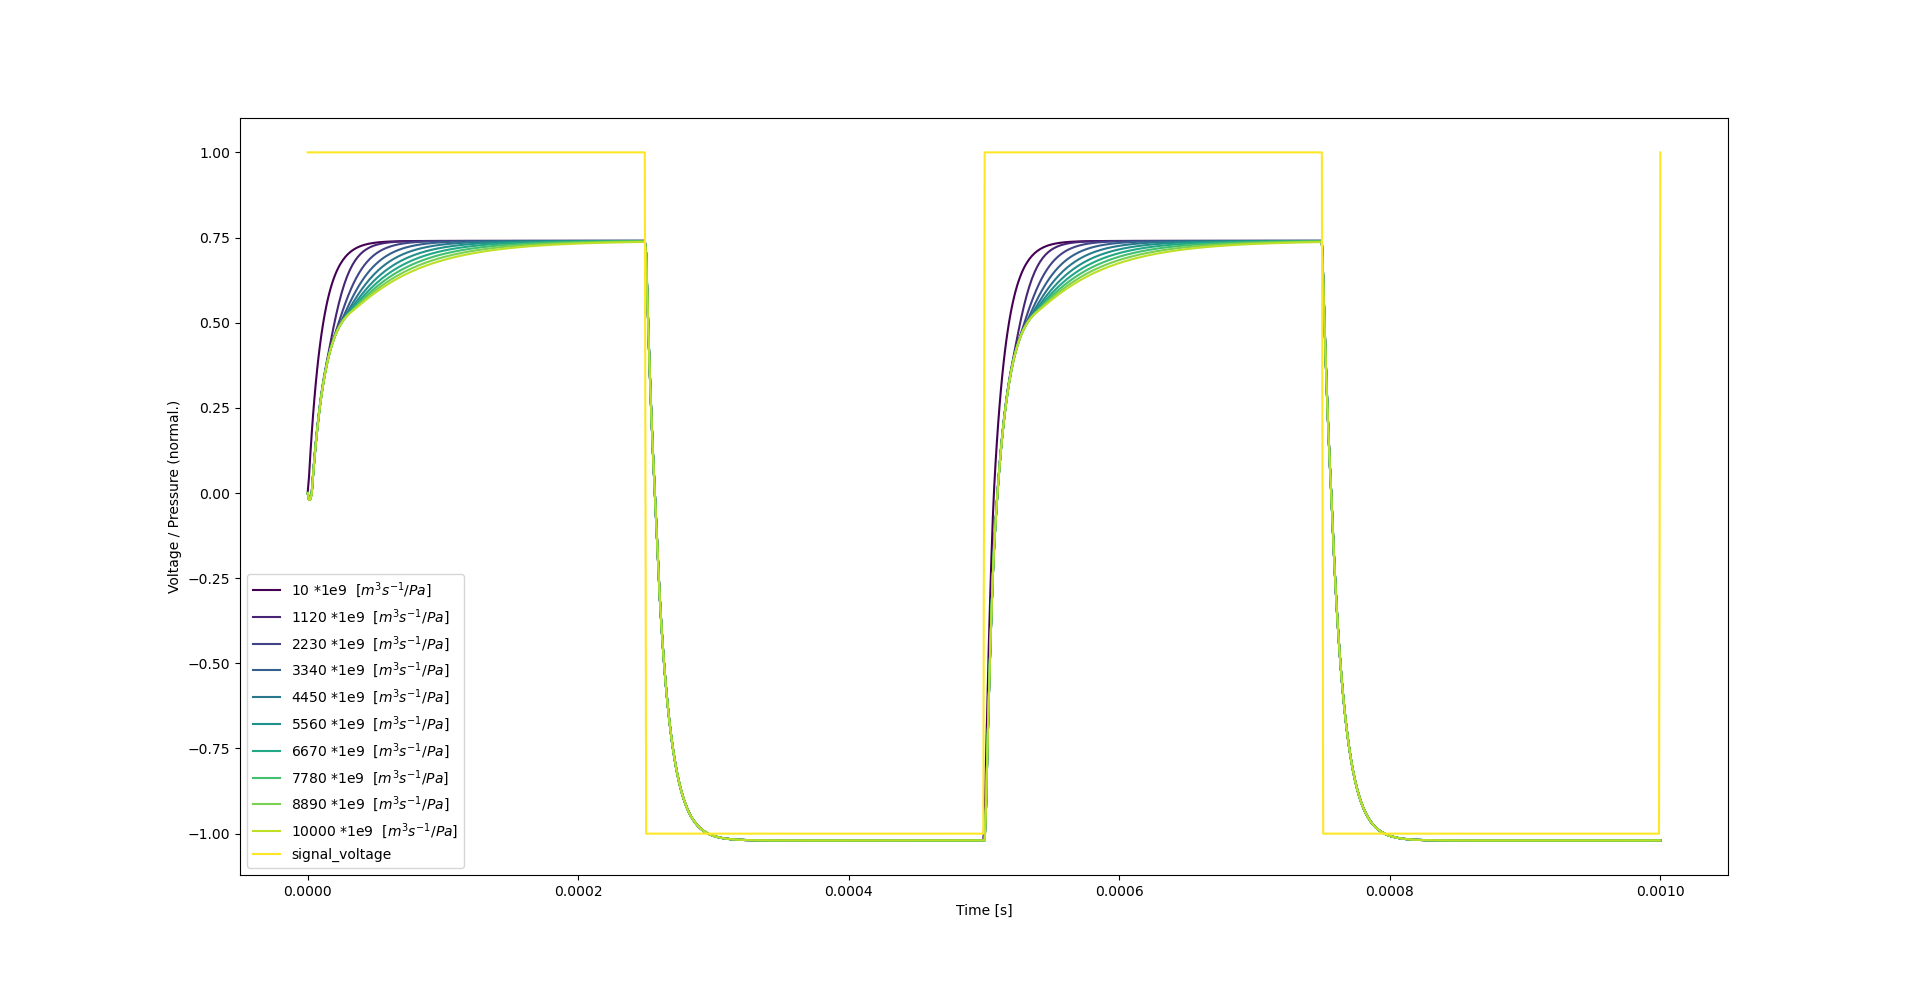
\includegraphics[width=\textwidth, valign=t]{bilder/velveresistance/vr_in_branch_multisweep.png}
		\caption{•}
	\end{subfigure}
	\caption{•}
\end{figure}

\begin{figure}[H]
	\centering
	\begin{subfigure}[H]{0.48\textwidth}
		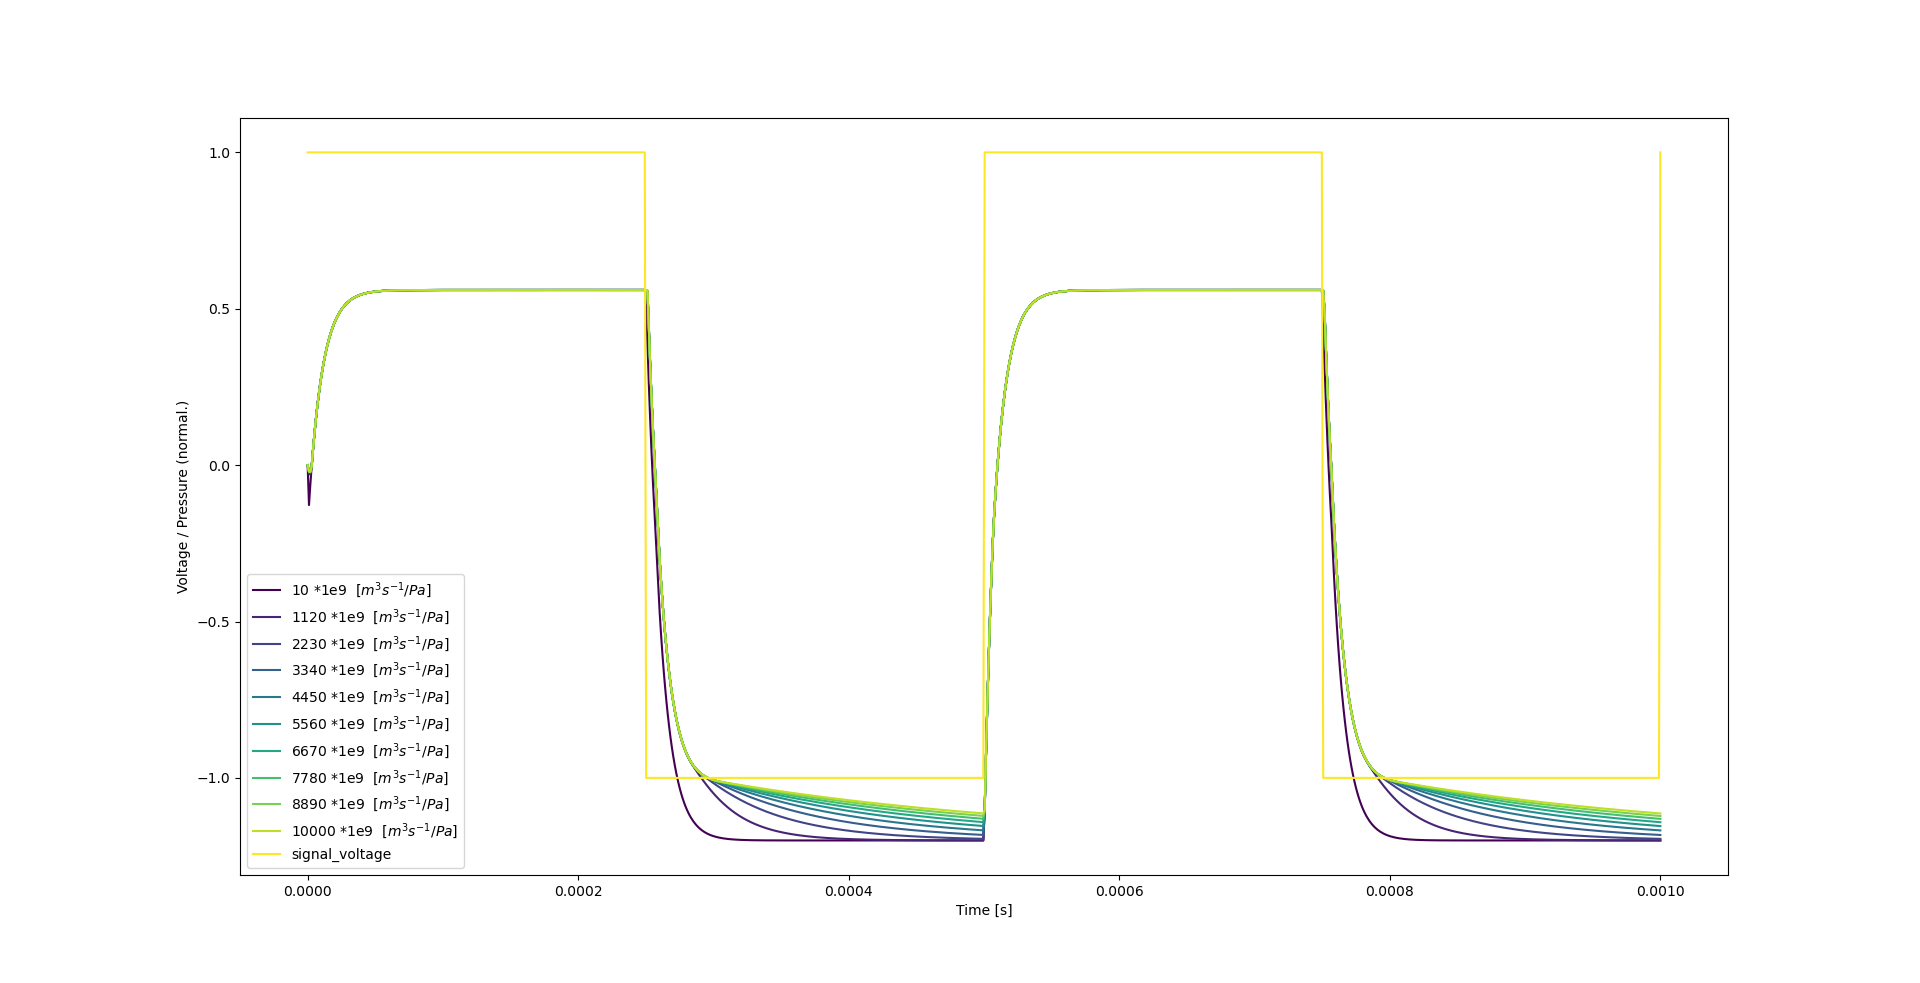
\includegraphics[width=\textwidth, valign=t]{bilder/velveresistance/vr_out_branch_multisweep.png}
		\caption{•}
	\end{subfigure}
	\begin{subfigure}[H]{0.48\textwidth}
		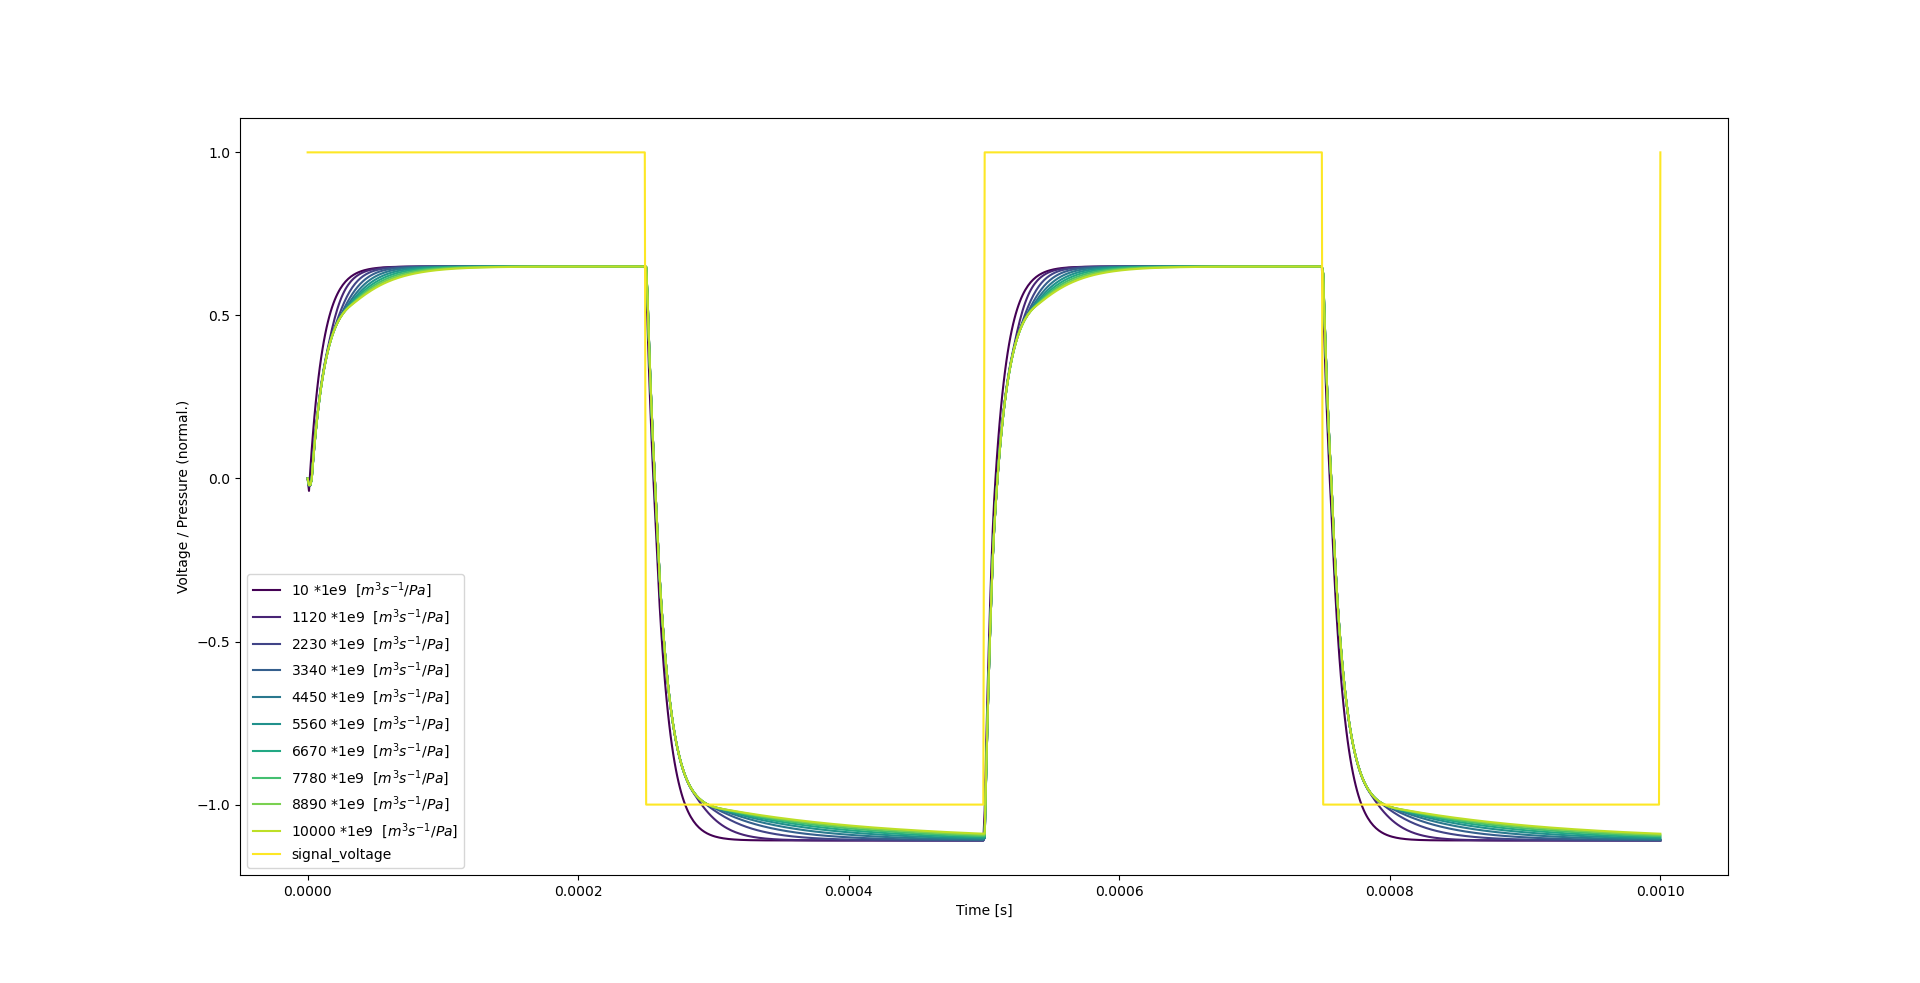
\includegraphics[width=\textwidth, valign=t]{bilder/velveresistance/vr_both_branch_multisweep.png}
		\caption{•}
	\end{subfigure}
	\caption{•}
\end{figure}

\subsection{Gegendruck}



\begin{figure}[H]
    \centering
    \begin{subfigure}[H]{0.48\textwidth}
        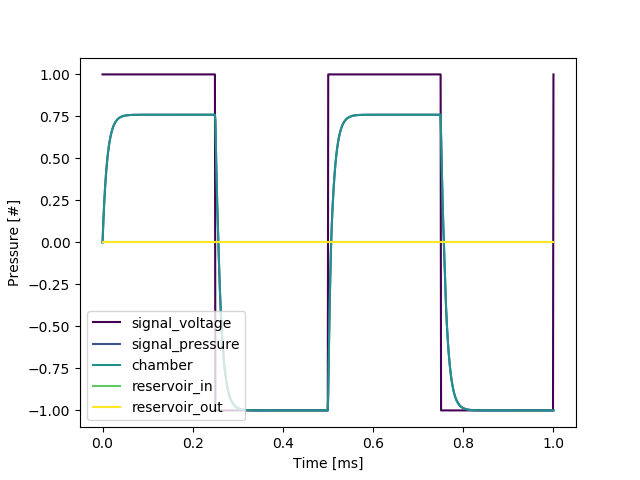
\includegraphics[width=\textwidth, valign=t]{bilder/backpressure/backpressure_free.png}
    \end{subfigure}
    \begin{subfigure}[H]{0.48\textwidth}
        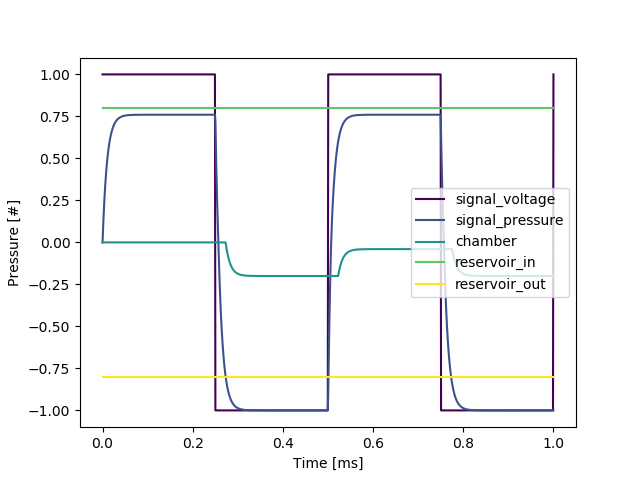
\includegraphics[width=\textwidth, valign=t]{bilder/backpressure/backpressure_example.png}
    \end{subfigure}
    \caption{a) Ohne externen Gegendruck b) Mit externem Gegendruck an Ein- und Auslass.}
\end{figure}

\begin{figure}[H]
    \centering
    \begin{subfigure}[H]{0.48\textwidth}
        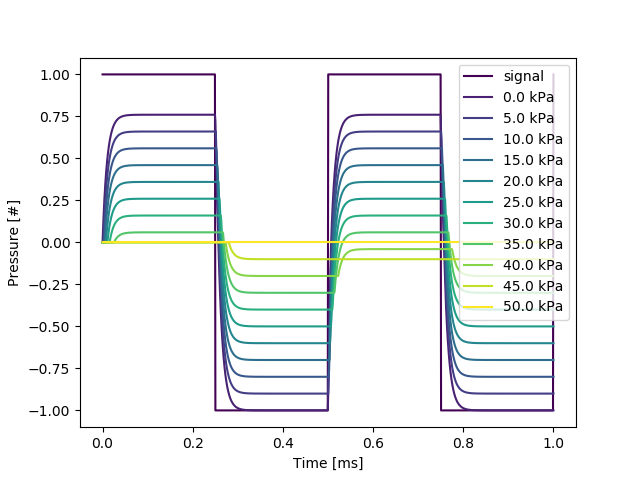
\includegraphics[width=\textwidth, valign=t]{bilder/backpressure/backpressure_at_pr_in_and_pr_out.png}
        \caption{•}
    \end{subfigure}
    \begin{subfigure}[H]{0.48\textwidth}
        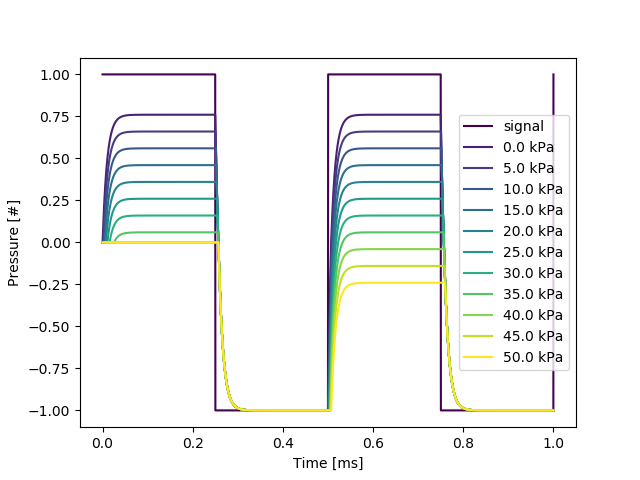
\includegraphics[width=\textwidth, valign=t]{bilder/backpressure/backpressure_at_pr_in.png}
        \caption{•}
    \end{subfigure}
    \caption{•}
\end{figure}

\begin{figure}[H]
	\centering
	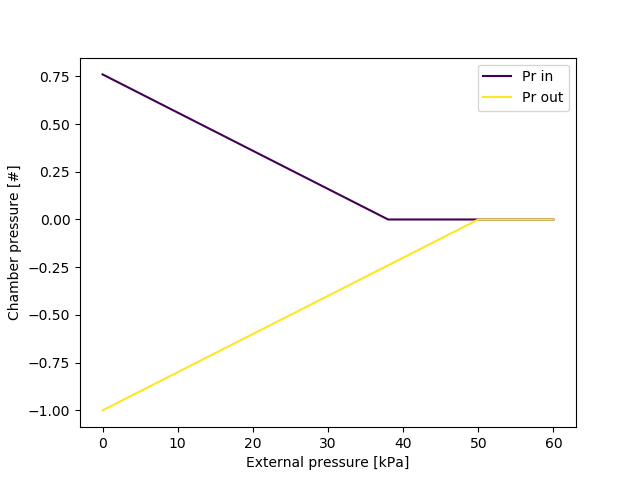
\includegraphics[width=0.7\textwidth]{bilder/backpressure/backpressure_result.png}
	\caption{•}
\end{figure}

\subsection{Grenzfrequenz}

\begin{figure}[H]
    \centering
    \begin{subfigure}[H]{0.48\textwidth}
        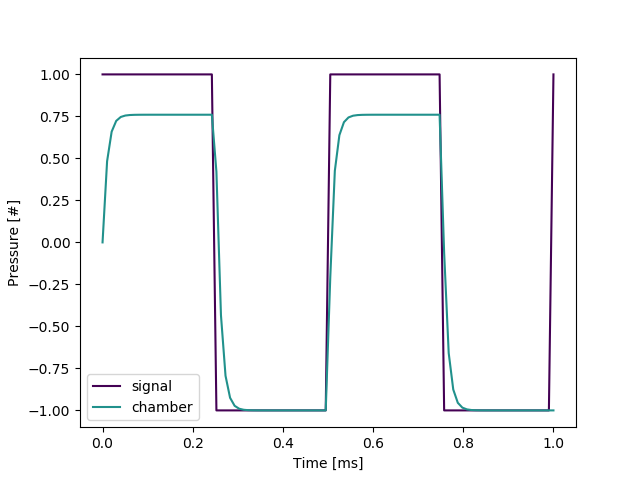
\includegraphics[width=\textwidth, valign=t]{bilder/frequency/frequency_default_2kHz.png}
        \caption{•}
    \end{subfigure}
    \begin{subfigure}[H]{0.48\textwidth}
        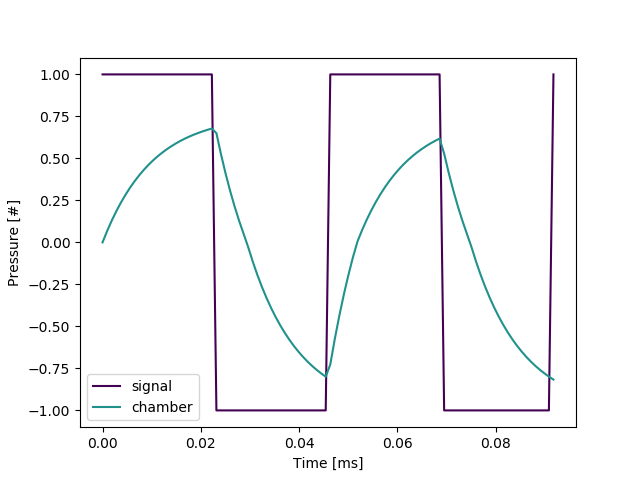
\includegraphics[width=\textwidth, valign=t]{bilder/frequency/frequency_to_fast_21_8 khz.png}
        \caption{•}
    \end{subfigure}
    \caption{•}
\end{figure}

\begin{figure}[H]
    \centering
    \begin{subfigure}[H]{0.48\textwidth}
        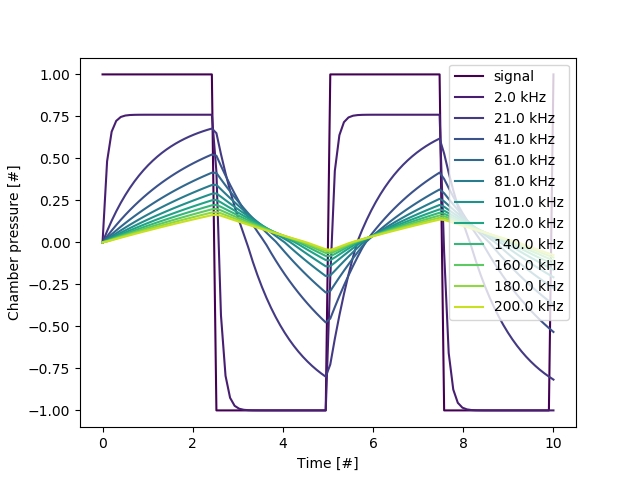
\includegraphics[width=\textwidth, valign=t]{bilder/frequency/frequency_sweep.png}
        \caption{•}
    \end{subfigure}
    \begin{subfigure}[H]{0.48\textwidth}
        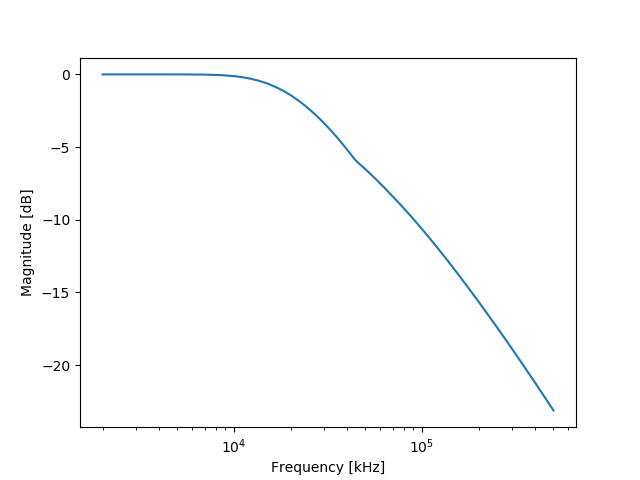
\includegraphics[width=\textwidth, valign=t]{bilder/frequency/bode_diagram.png}
        \caption{•}
    \end{subfigure}
    \caption{•}
\end{figure}

\section{Fazit}

\section{Ausblick}

Das Systemmodell kann hinsichtlich der einzelnen Komponenten nahezu beliebig komplex erweitert werden. Um einen Einblick zu erlangen, welche Konsequenzen ein höherer Detailierungsgrad nach sich zieht, wird die Beschreibung der Ventile und der Rohrleitungen erweitert. Das Ventil besitzt durch die zugrundeliegende Geometrie auch kapazitive Eigenschaften, verursacht durch elastische Verformungen des Bauteils. Dieser Effekt wird im folgenden Modell durch parallele Kondensatoren ($C_{V_{in}}$ und $C_{V_{out}}$) berücksichtigt. Zusätzlich kann der Fluid-inherente Widerstand gegen Beschleunigungen innerhalb von Rohrleitungen durch eine Induktivität ($L_{V_{in}}$ und $L_{V_{out}}$) beschrieben werden. Dabei gilt folgende elektro-fluidische Analogie:


\begin{equation}
	L_{fluid} = \frac{P}{\ddot{V}} \:\:\widehat{=}\:\: L_{elek.} = \frac{U}{dI/dt}
\end{equation}

\begin{equation}
	I_{C} = I_{in} + I_{out}
\end{equation}

\begin{center}
	\includesvg[scale = 0.6]{bilder/circuits/second_order_circuit}
\end{center}

Eine Herleitung der Differentialgleichung für dargestelltes System führt zu folgendem Zusammenhang nach Trennung der Variablen:


\begin{equation}
	\begin{split}
		&+ \left[\left(1+\frac{R_{T_{out}}}{R_{V_{out}}}\right)C_{V_{in}}L_{T_{in}}C_{C}\right]\bm{\frac{d\textsuperscript{3}U_{C}}{dt\textsuperscript{3}}} \\
		&+ \left[\left(1+\frac{R_{T_{out}}}{R_{V_{out}}}\right)C_{V_{in}}R_{C}C_{C} + \left(1+\frac{R_{T_{in}}}{R_{V_{in}}}\right)C_{V_{out}}R_{C}C_{C}\right]\bm{\frac{d\textsuperscript{2}U_{C}}{dt\textsuperscript{2}}} \\
		&+ \biggl[\left(1+\frac{R_{T_{in}}}{R_{V_{in}}}\right)\left(1+\frac{R_{T_{out}}}{R_{V_{out}}}\right)C_{C} + \left(1+\frac{R_{T_{out}}}{R_{V_{out}}}\right)\left(\frac{R_{C}C_{C}}{R_{V_{in}}}+C_{V_{in}}\right) + \\
		& \left(1+\frac{R_{T_{in}}}{R_{V_{in}}}\right)\left(\frac{R_{C}C_{C}}{R_{V_{out}}}+C_{V_{out}}\right)\biggr] \bm{\frac{dU_{C}}{dt}}  \\
		&+ \left[\left(1+\frac{R_{T_{out}}}{R_{V_{out}}}\right)\frac{1}{R_{V_{out}}} + \left(1+\frac{R_{T_{in}}}{R_{V_{in}}}\right)\frac{1}{R_{V_{out}}}\right]\bm{U_{C}} \\
		&= \biggl[\left(1+\frac{R_{T_{out}}}{R_{V_{out}}}\right)\left(\frac{L_{T_{in}}}{R_{V_{in}}}+C_{V_{in}}R_{V_{in}}\right) - \left(1+\frac{R_{T_{in}}}{R_{V_{in}}}\right)\left(\frac{L_{T_{out}}}{R_{V_{out}}}+C_{V_{out}}R_{V_{out}}\right)\biggr]\bm{\frac{dI_{out}}{dt}} \\
		&+ \left[\left(1+\frac{R_{T_{out}}}{R_{V_{out}}}\right)C_{V_{in}}L_{T_{in}} - \left(1+\frac{R_{T_{in}}}{R_{V_{in}}}\right)C_{V_{out}}L_{T_{out}}\right]\bm{\frac{d\textsuperscript{2}I_{out}}{dt\textsuperscript{2}}} \\
		&+ \left(1+\frac{R_{T_{out}}}{R_{V_{out}}}\right)\frac{1}{R_{T_{in}}}\bm{(U_{Signal}(t) - U_{in})}+ \left(1+\frac{R_{T_{out}}}{R_{V_{out}}}\right)C_{V_{in}}\bm{\frac{d(U_{Signal}(t) - U_{in})}{dt}} \\
		&+ \left(1+\frac{R_{T_{in}}}{R_{V_{in}}}\right)\frac{1}{R_{T_{out}}}\bm{(U_{Signal}(t) - U_{out})} + \left(1+\frac{R_{T_{in}}}{R_{V_{in}}}\right)C_{V_{out}}\bm{\frac{d(U_{Signal}(t) - U_{out})}{dt}}
	\end{split}
\end{equation}

%\[ L_{fluid} = \frac{P}{\ddot{V}} \:\:\widehat{=}\:\: L_{elek.} = \frac{U}{dI/dt} \]

Es ist ersichtlich, dass die Simulation in dieser Detailierung den Rahmen dieser Arbeit übersteigt.


\printbibliography

\end{document}
